%%%%%%%%%%%%%%%%%%%%%%%%%%%%%%%%%%%%%%%%%%
% Engineering problems / LaTeX Template
%		Semester 6
%		Institut d'Optique Graduate School
%%%%%%%%%%%%%%%%%%%%%%%%%%%%%%%%%%%%%%%%%%
%	6N-IntNum-BlocRobot	/ Embedded System
%%%%%%%%%%%%%%%%%%%%%%%%%%%%%%%%%%%%%%%%%%
%
% Created by:
%	Julien VILLEMEJANE - 19/oct/2024	
%
%%%%%%%%%%%%%%%%%%%%%%%%%%%%%%%%%%%%%%%%%%
% Professional Newsletter Template
% LaTeX Template
% Version 1.0 (09/03/14)
%
% Created by:
% Bob Kerstetter (https://www.tug.org/texshowcase/) and extensively modified by:
% Vel (vel@latextemplates.com)
% 
% This template has been downloaded from:
% http://www.LaTeXTemplates.com
%
% License:
% CC BY-NC-SA 3.0 (http://creativecommons.org/licenses/by-nc-sa/3.0/)
%
%%%%%%%%%%%%%%%%%%%%%%%%%%%%%%%%%%%%%%%%%

\documentclass[a4paper,11pt,titlepage]{article} % The default font size is 10pt; 11pt and 12pt are alternatives

%%%%%%%%%%%%%%%%%%%%%%%%%%%%%%%%%%%%%%%%%%%%%%%%%%%%%%%%%%%%%%%%%%%%%%%%%%%%%%%%%%%%%%%%%%%%%%%%%%%%%%%%%%%%%%%%%%%%%%%%%%%%%%%%%%%%%%%%%%%%%%%%%%%%%%%%%%%%%%%%%%%%%%%%%%%%%%%%%%%%%%%%%%%%%%%%%%%%%%%%%%%%%%%%%%%%%%%%%%%%%%%%%%%%%%%%%%%%%%%%%%%%%%%%%%%%
\usepackage{opto_elec_villemejane}

%%%%%%%%%%%%%%%%%%%%%%%%%%%%%%%%%%%%%%%%%%%%%%%%
%%%%%%%%%%%%%%%%%%%%%%%%%%%%%%%%%%%%%%%%%%%%%%%%
\begin{document}



% Page de garde
\begin{titlepage}

\begin{center}
	\begin{minipage}{2.5cm}
	\begin{center}
		
\includegraphics[width=8cm]{images/Logo-LEnsE.png}
	\end{center}
\end{minipage}\hfill
\begin{minipage}{10cm}
	\begin{center}
	\textbf{Institut d'Optique Graduate School }\\[0.1cm]
    \textbf{Interfaçage Numérique}


	\end{center}
\end{minipage}\hfill


\vspace{4cm}


{\huge \bfseries \textsc{Interfaçage Numérique}} \\[0.5cm]
{\large \bfseries Travaux Pratiques} \\[0.2cm]
Semestre 6

\vspace{2cm}
% Title
\rule{\linewidth}{0.3mm} \\[0.4cm]
{ \huge \bfseries\color{violet_iogs} Robotique et systèmes embarqués\\[0.4cm] }
\rule{\linewidth}{0.3mm} \\[1cm]

4 séances

\bigskip

\begin{center}
	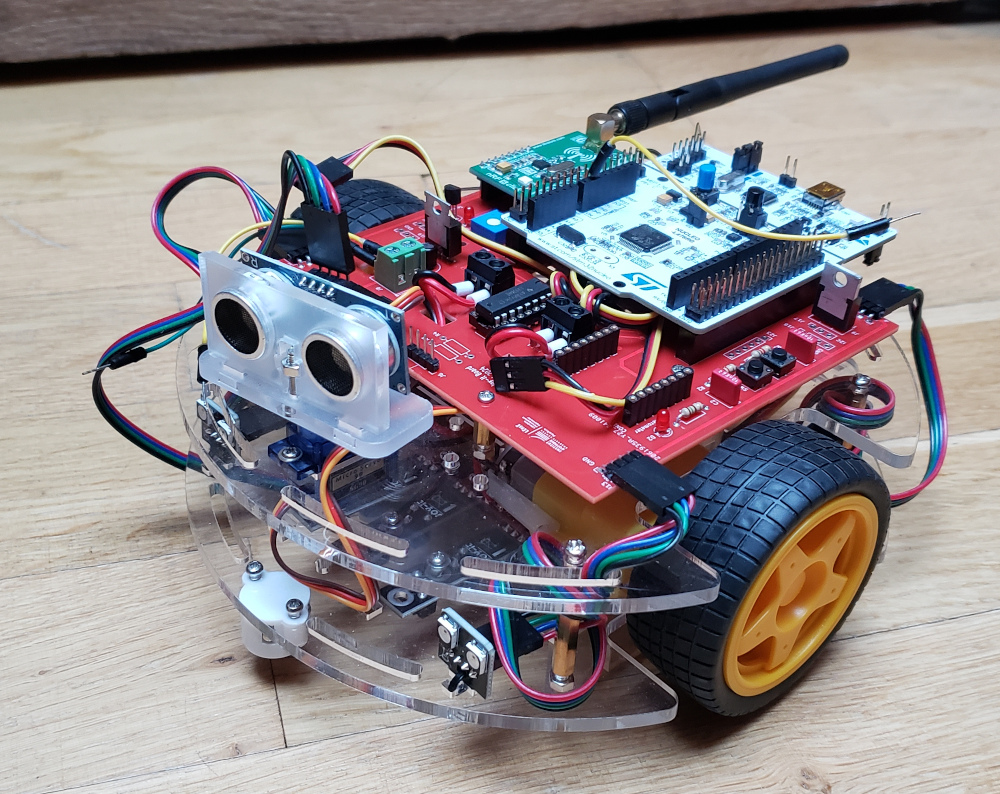
\includegraphics[width=0.4\textwidth]{images/robot_joycar.jpg}
\end{center}

\vfill

\textit{Ce sujet est disponible au format électronique sur le site du LEnsE - https://lense.institutoptique.fr/ dans la rubrique Année / Première Année / Interfaçage Numérique S6 / Robotique.}

% Bottom of the page
%{\textbf{\large {Année universitaire} 2024-2025}}

\end{center}
\end{titlepage}

\newpage
\strut % empty page


%%%%%%%%%%%%%%%%%%%%%%%%%%%%%%%%%%%%%%%%%%%%%%%%
%%%%%%%%%%%%%    Intro
\newpage
\pagestyle{empty}

\begin{minipage}[c]{.25\linewidth}
	
\includegraphics[width=5cm]{images/Logo-LEnsE.png}
\end{minipage} \hfill
\begin{minipage}[c]{.4\linewidth}

\begin{center}
\vspace{0.3cm}
{\Large \textsc{Interfaçage Numérique}}

\medskip

6N-047-SCI \qquad \textbf{\Large Bloc Robot}

\end{center}
\end{minipage}\hfill

\vspace{0.5cm}

\noindent \rule{\linewidth}{1pt}

{\noindent\Large  \rule[-7pt]{0pt}{30pt} \textbf{Robotique et systèmes embarqués}}

\noindent \rule{\linewidth}{1pt}

\bigskip 

%%%%%%%%%%%%%%%%%%%%%%%%%%%%%%%%%%%%%%%%%%%%%%%%
%%%%%%%%%%%%%    A A V

{\large À l'issue des séances de TP concernant le \textbf{bloc de robotique}, les étudiant$\cdot$es seront capables de :}

\medskip

\begin{itemize}
	\item Développer et mettre en \oe{}uvre une \textbf{solution d'électronique embarquée} pour \textbf{mettre en mouvement un robot}
	\item Concevoir un \textbf{programme embarqué} permettant de \textbf{rendre autonome les mouvements d'un robot}
\end{itemize}

\noindent \rule{\linewidth}{1pt}


%%%%%%%%%%%%%%%%%%%%%%%%%%%%%%%%%%%%%%%%%%%%%%%%
%%%%%%%%%%%%%    Objectifs

\section{Objectifs du mini-projet}

L'objectif principal de ce mini-projet est de \textbf{développer le code embarqué d'une plateforme robotique} lui permettant de se déplacer de manière autonome le long d'une ligne sans percuter d'obstacle.
%	\item soit d'être piloter à distance par une télécommande et d'afficher des informations provenant de capteurs intégrés à la plateforme.  Pour 2025-2026 !!

\begin{center}
	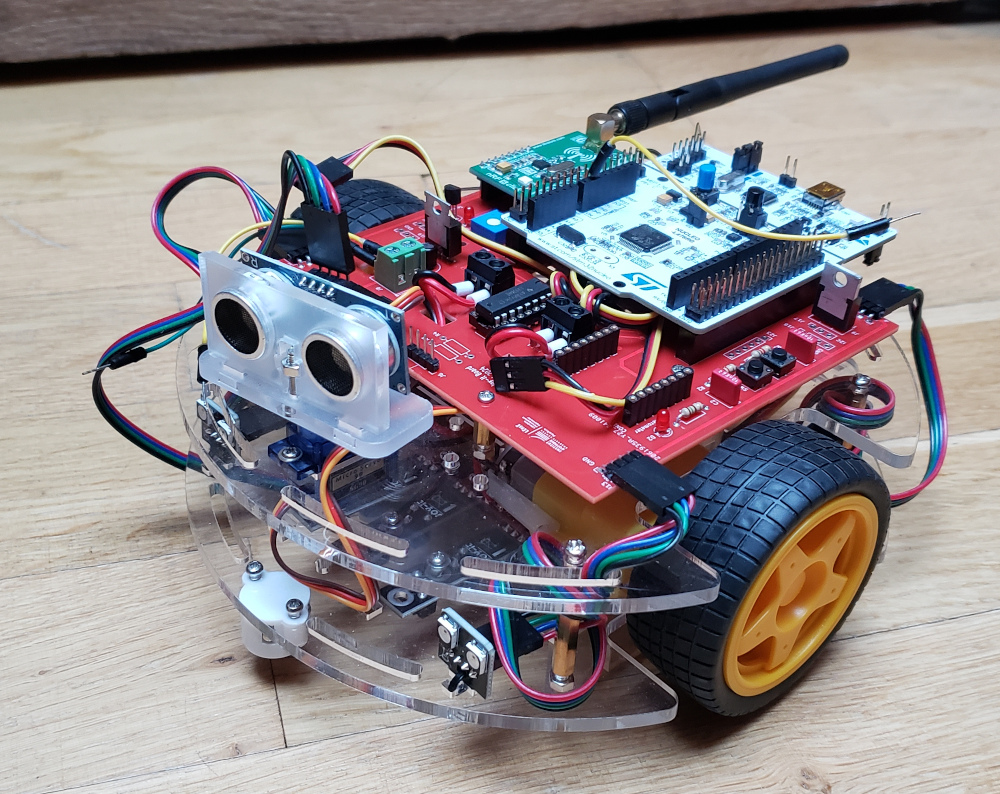
\includegraphics[width=0.4\textwidth]{images/robot_joycar.jpg}
\end{center}


\medskip

Vous aurez à votre disposition une \textbf{maquette} basée sur un robot Joy-It Car. Cette maquette est pilotée par une carte Nucléo (contenant un microcontroleur).


\newpage
%%%%%%%%%%%%%%%%%%%%%%%%%%%%%%%%%%%%%%%%%%%%%%%%
%%%%%%%%%%%%%    Déroulement

\section{Déroulement du bloc}

\textit{La liste des étapes à suivre pour la réalisation du programme embarqué de la plateforme de rayonnement lumineux est donnée à titre indicatif. L'ordre et le choix des différentes étapes sont laissés à l'appréciation des différents binômes.}

\textit{Afin de faciliter la réutilisation des codes, il pourra être intéressant de définir des fonctions pour le pilotage des différents éléments.}

\subsection{Séance 1 / Arduino et Nucléo-STM32 (sans maquette !!)}

\textit{Le sujet de cette séance est fourni dans un document annexe, disponible aussi sur le site du LEnsE - https://lense.institutoptique.fr/ dans la rubrique Année / Première Année / Interfaçage Numérique S6 / Bloc Systèmes embarqués / Intro Arduino et STM32.}

	\begin{description}
		\item[Etape 0 - 30 min] Installer les drivers STM32 et tester un premier programme
		\item[Etape 1 - 45 min] Piloter des sorties numériques - LED
		\item[Etape 2 - 45 min] Acquérir des données numériques - Bouton-poussoirs
		\item[Etape 3 - 45 min] Mettre en \oe{}uvre des interruptions sur des événements externes
		\item[Etape 4 - 45 min] Utiliser des sorties modulées en largeur d'impulsion (PWM) - LEDs
		\item[Etape 5 - 60 min] Acquérir des données analogiques - Potentiomètre
	\end{description}	


\subsection{Séance 2 / Prise en main de la maquette et déplacements élémentaires}

	\begin{description}
		\item[Etape 6 - 60 min] Piloter l'intensité des LEDs de la maquette
		\item[Etape 7 - 90 min] Piloter les moteurs à courant continu
		\item[Etape 8 - 60 min] Acquérir des données des capteurs de ligne				\item[Etape 9 - 60 min] Piloter les phares du robot à l'aide de la bibliothèque WS2812 (NeoPixel)
	\end{description}


\subsection{Séances 3 et 4 - Pilotage de haut niveau}

Les deux séances suivantes seront consacrées au pilotage du robot pour lui permettre de suivre une ligne ou/et d'éviter les obstacles qu'il rencontre sur son chemin.

Les étapes possibles sont les suivantes :

\begin{description}
	\item[Etape 10 - 120 min] Définir et tester une première structure de code permettant de piloter les deux moteurs du robot en fonction de la détection des lignes
	\item[Etape 11 - 90 min] Acquérir les signaux du capteur ultrason
	\item[Etape 12 - 90 min] Piloter le servomoteur associé au capteur ultrason
	\item[Etape 13 - 180 min] Améliorer le programme de contrôle du robot
\end{description}

Vous pourrez également ajouter d'autres éléments présents sur la carte : encodeur de vitesse sur les roues, capteurs de température (analogique ou numérique en I2C), accéléromètre (I2C).



\newpage
\strut % empty page
%%%%%%%%%%%%%%%%%%%%%%%%%%%%%%%%%%%%%%%%%%%%%%%%
%%%%%%%%%%%%%    Séance 2 détaillée
\begin{minipage}[c]{.25\linewidth}
	
\includegraphics[width=4cm]{images/Logo-LEnsE.png}
\end{minipage} \hfill
\begin{minipage}[c]{.4\linewidth}

\begin{center}
\vspace{0.3cm}
{\Large \textsc{Interfaçage Numérique}}

\medskip

6N-047-SCI \qquad \textbf{\Large Bloc Robot}

\end{center}
\end{minipage}\hfill

\vspace{0.5cm}

\noindent \rule{\linewidth}{1pt}

{\noindent\Large \rule[-7pt]{0pt}{30pt} \textbf{Séance 2} / Prise en main de la maquette et déplacements élémentaires} 

\noindent \rule{\linewidth}{1pt}




	\begin{description}
		\item[Etape 6 - 60 min] Piloter l'intensité des LEDs de la maquette
		\item[Etape 7 - 90 min] Piloter les moteurs à courant continu
		\item[Etape 8 - 60 min] Acquérir des données des capteurs de ligne				\item[Etape 9 - 60 min] Piloter les phares du robot à l'aide de la bibliothèque WS2812 (NeoPixel)
	\end{description}




%%%%%%%%%%%%%%%%%%%%%%%%%%%%%%%%%%%%%%%%%%%%%%%%
%%%%%%%%%%%%%    Objectifs
\section{Objectifs de la séance}

Cette seconde séance est consacrée à la \textbf{prise en main de la maquette} et au développement des \textbf{fonctionnalités permettant les déplacements élémentaires} de la plateforme.


%%%%%%%%%%%%%%%%%%%%%%%%%%%%%%%%%%%%%%%%%%%%%%%%
%%%%%%%%%%%%%    Maquette
\section{Description de la maquette}


\subsection{Eléments constitutifs}



\subsection{Alimentation électrique}


\noindent \rule{\linewidth}{1pt}

\bigskip

{\LARGE La tension maximale admissible par les moteurs est de $7\operatorname{V}$ !}

\bigskip

\noindent \rule{\linewidth}{1pt}


\subsection{Brochage}

\subsubsection{Entrées-Sorties standard}

\begin{center}
\begin{tabular}{|l|l|l|l|}
\hline 
Maquette & \textbf{Broche Nucléo} & Type & Description \\ 
\hline 
\textsc{LED1} & PC7 & Sortie / PWM & Led active à l'\textbf{état haut}\\ 
\textsc{LED2} & PB13 & Sortie / PWM & Led active à l'\textbf{état bas}\\ 
\hline 
\textsc{SW1} & PA11 & Entrée & Bouton-poussoir, par défaut état bas\\ 
\textsc{SW2} & PA12 & Entrée & Bouton-poussoir, par défaut état bas\\ 
\textsc{UserButton} & PC13 & Entrée & Bouton-poussoir, par défaut état haut\\
\hline  
\textsc{POT\_OUT} & PC3 & Entrée analogique & Potentiomètre\\
\hline  
\end{tabular} 
\end{center}

\subsubsection{Moteurs}

\begin{center}
\begin{tabular}{|l|l|l|l|}
\hline 
Maquette & \textbf{Broche Nucléo} & Type & Description \\ 
\hline 
\textsc{MOT\_EN} & PA9 & Sortie & Validation des moteurs\\ 
\hline 
\textsc{MOT\_L\_1} & PB4 & Sortie / PWM & Moteur Gauche direction 1\\ 
\textsc{MOT\_L\_2} & PA8 & Sortie / PWM & Moteur Gauche direction 2\\ 
\hline 
\textsc{MOT\_R\_1} & PA0 & Sortie / PWM & Moteur Droit direction 1\\ 
\textsc{MOT\_R\_2} & PA1 & Sortie / PWM & Moteur Droit direction 2\\ 
\hline  
\end{tabular} 
\end{center}

\subsubsection{Phares NeoPixel / SW2812}

\begin{center}
\begin{tabular}{|l|l|l|l|}
\hline 
Maquette & \textbf{Broche Nucléo} & Type & Description \\ 
\hline 
\textsc{Din\_1} & PC0 & Sortie & Phare avant droit\\ 
\textsc{Din\_2} & PA10 & Sortie & Phare avant gauche\\ 
\textsc{Din\_3} & PC5 & Sortie & Phare arrière gauche\\ 
\textsc{Din\_4} & PA13 & Sortie & Phare arrière droit\\ 
\hline  
\end{tabular} 
\end{center}

\subsubsection{Capteurs}

\begin{center}
\begin{tabular}{|l|l|l|l|}
\hline 
Maquette & \textbf{Broche Nucléo} & Type & Description \\ 
\hline 
\textsc{TEMP\_OUT} & PC2 & Entrée analogique & Capteur de température MCP9700\\ 
\hline 
\textsc{Line\_L} & PA7 & Entrée & Capteur de ligne Gauche\\ 
\textsc{Line\_C} & PB6 & Entrée & Capteur de ligne Centre\\ 
\textsc{Line\_R} & PA5 & Entrée & Capteur de ligne Droit\\ 
\hline 
\textsc{Speed\_L} & PC9 & Entrée & Vitesse moteur Gauche\\ 
\textsc{Speed\_R} & PC8 & Entrée & Vitesse moteur Droit\\ 
\hline  
\textsc{US\_trig} & PB5 & Sortie & Capteur ultrason - Trig\\ 
\textsc{US\_echo} & PB3 & Entrée & Capteur ultrason - Echo\\ 
\textsc{Servo} & PB7 & Sortie / PWM & Servomoteur du capteur Ultrason\\ 
\hline  
\end{tabular} 
\end{center}


\subsubsection{Accéléromètre / MikroE-6DOF IMU 3 Click}

Ce module fonctionne à l'aide du protocole I2C.

\begin{center}
\begin{tabular}{|l|l|l|l|}
\hline 
Maquette & \textbf{Broche Nucléo} & Type & Description \\ 
\hline 
\textsc{SDA} & PB9 & Entrée-Sortie & Signal de données bidirectionnel \\ 
\textit{SCL} & PB8 & Sortie & Signal d'horloge\\
\hline 
\textsc{Reset} & PC4 & Sortie & Reset matériel du composant\\ 
\textit{Interrupt} & PB10 & Entrée & Interruption sur réception\\ 
\hline 
\end{tabular} 
\end{center}

\subsubsection{Capteur température numérique / TC74A2}

Ce module fonctionne à l'aide du protocole I2C.

\begin{center}
\begin{tabular}{|l|l|l|l|}
\hline 
Maquette & \textbf{Broche Nucléo} & Type & Description \\ 
\hline 
\textsc{SDA} & PB9 & Entrée-Sortie & Signal de données bidirectionnel \\ 
\textit{SCL} & PB8 & Sortie & Signal d'horloge\\
\hline 
\end{tabular} 
\end{center}


\subsubsection{Communication nRF24L01}

Ce module fonctionne selon le protocole SPI. \textit{Il doit nécessairement être utilisé avec un second module afin de pouvoir transmettre des données entre deux microcontroleurs.}

\begin{center}
\begin{tabular}{|l|l|l|l|}
\hline 
Maquette & \textbf{Broche Nucléo} & Type & Description \\ 
\hline 
\textsc{SPI} & & & \\ 
\textit{SCK} & PC10 & Sortie & Signal d'horloge\\
\textit{MISO} & PC11 & Entrée & Données entrantes\\
\textit{MOSI} & PC12 & Sortie & Données sortantes\\ 
\hline  
\textit{CS} & PA14 & Sortie & Sélection du composant\\ 
\textit{CE} & PD2 & Sortie & Validation du composant (puissance)\\ 
\textit{INT} & PA15 & Entrée & Interruption sur réception\\ 
\hline  
\end{tabular} 
\end{center}


\subsubsection{Utilisation de la sortie modulée PB7}
	
\begin{lstlisting}
LL_GPIO_SetAFPin_0_7(GPIOB,  GPIO_PIN_7,  GPIO_AF1_TIM2);
\end{lstlisting}





\newpage


\section{Etape 9 - Acquérir des données de l'accéléromètre (I2C)}

\begin{center} \textbf{\textit{Temps conseillé : 90 min}} \end{center}

Le composant que nous allons étudier est un \textbf{accéléromètre et magnétomètre} intégrés sur une même puce de silicium. Sa référence est \textbf{FXOS8700CQ}. Ce composant est intégré au module \textit{MikroE} \textbf{DOF6 - IMU Click}.

\subsection{Protocole I2C}

DESCRIPTION PROTOCOLE et CONNECTIQUES !

\bigskip

\textsc{Attention !} Les broches utilisées sur la carte Nucléo pour l'I2C ne sont pas celles par défaut. Il est indispensable de préciser les broches SDA et SCL à l'aide des méthodes suivantes :

\begin{lstlisting}
Wire.setSDA( PB9 );    
Wire.setSCL( PB8 ); 
\end{lstlisting}

\bigskip

\Manip Ouvrir le code \textsl{09\_accelero.ino} fourni. Compiler ce code et téléverser ce code dans la carte Nucléo.

Ce code contient les fonctions \textsl{test\_FXOS()} et \textsl{read\_i2c\_buffer()}, ainsi que des définitions des registres internes du composant.

\Manip 

\subsection{Configuration}


\subsection{Récupération des données}

\textit{These registers contain the X-axis, Y-axis, and Z-axis 14-bit left-justified sample data expressed as 2's complement numbers.} [NXP Doc p.52 of 113] 

\subsection{Traceur Série}

\begin{lstlisting}
  Serial.print(valeur1);
  Serial.print(",");
  Serial.print(valeur2);
  Serial.print(",");
  Serial.print(valeur3);
  Serial.print(",");
  Serial.print(valeur4);
  Serial.println();
\end{lstlisting}



%%%%%%%%%%%%%%%%%%%%%%%%%%%%%%%%%%%%%%%%%%%%%%%%
%%%%%%%%%%%%%    Présentation de la maquette
\newpage
\begin{minipage}[c]{.25\linewidth}
	
\includegraphics[width=4cm]{images/Logo-LEnsE.png}
\end{minipage} \hfill
\begin{minipage}[c]{.4\linewidth}

\begin{center}
\vspace{0.3cm}
{\Large \textsc{Interfaçage Numérique}}

\medskip

6N-047-SCI \qquad \textbf{\Large Bloc Robot}

\end{center}
\end{minipage}\hfill

\vspace{0.5cm}

\noindent \rule{\linewidth}{1pt}

{\noindent\Large \rule[-7pt]{0pt}{30pt} \textbf{Robot Joy-It Car} / Présentation du matériel}

\noindent \rule{\linewidth}{1pt}

\bigskip

{\LARGE La tension maximale admissible par les moteurs est de $7\operatorname{V}$ !}

\bigskip

\noindent \rule{\linewidth}{1pt}


%%%%%%%%%%%%%%%%%%%%%%%%%%%%%%%%%%%%%%%%%%%%%%%%
%%% RESSOURCES COMPLEMENTAIRES		

\newpage
% Ressources
\begin{center}
	\begin{minipage}{2.5cm}
	\begin{center}
		
\includegraphics[width=5cm]{images/Logo-LEnsE.png}
	\end{center}
\end{minipage}\hfill
\begin{minipage}{10cm}
	\begin{center}
	\textbf{Institut d'Optique Graduate School }\\[0.1cm]
    \textbf{Interfaçage Numérique}


	\end{center}
\end{minipage}\hfill


\vspace{2cm}


{\Large \bfseries \textsc{Interfaçage Numérique}} \\[0.5cm]
{\large \bfseries Travaux Pratiques} \\[0.2cm]
Semestre 6

\vspace{1cm}

% Title
\rule{\linewidth}{0.4mm} \\[0.4cm]
{ \Large \bfseries\color{violet_iogs} Ressources \\[0.4cm] }
\rule{\linewidth}{0.4mm} \\[1cm]
{\large Bloc Robot}

\end{center}

\vspace{3cm}

\textbf{\large Liste des ressources}
\begin{itemize}
	\item \hyperref[doc:robot_schematic]{Schéma de la carte du robot Joy-It Car}
	\item \hyperref[doc:robot_pcb]{PCB de la carte du robot Joy-It Car}
\end{itemize}

\vfill

\newpage
\strut % empty page
% Ressources
\titleformat{\section}
  {\null}{}{0pt}{}


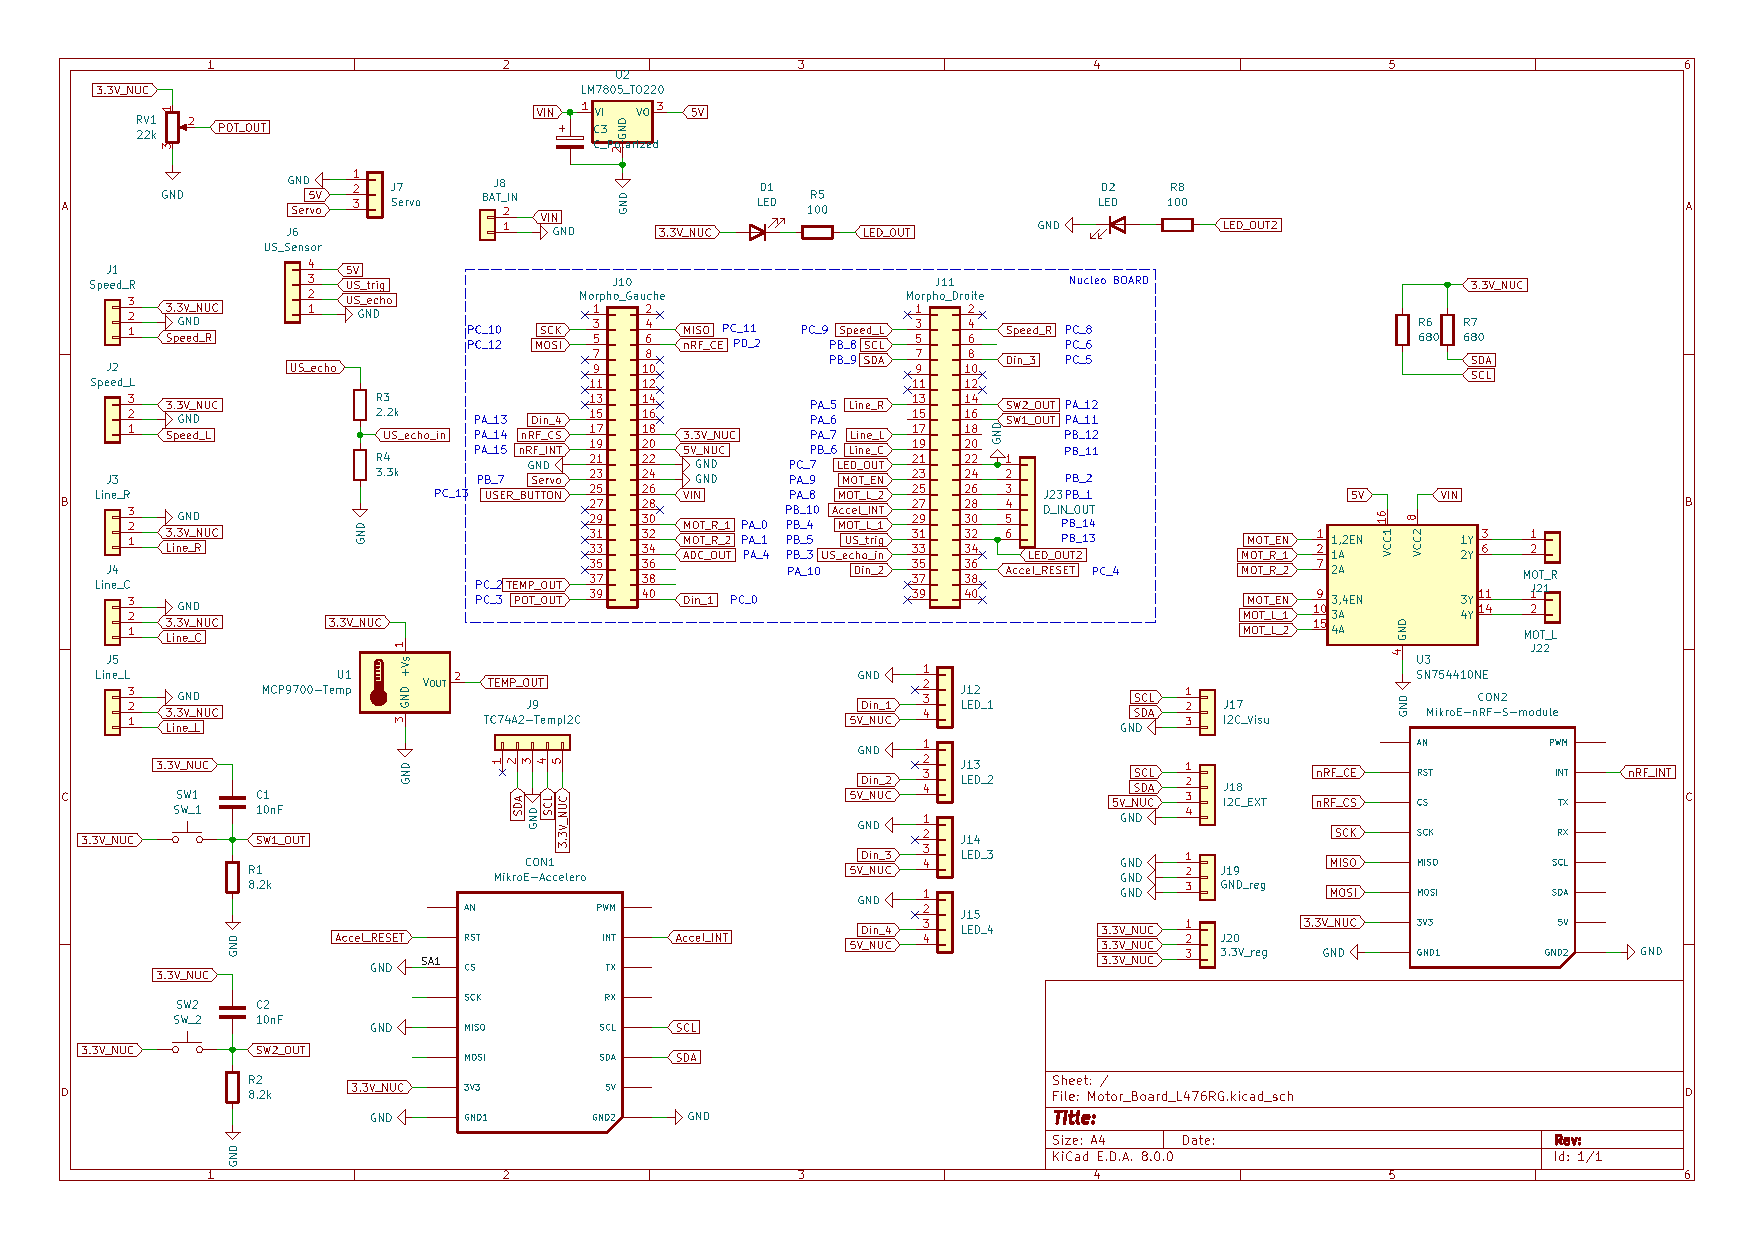
\includepdf[pages=1, landscape=true, pagecommand={\section{\texorpdfstring{\hspace{-1em}}{Schéma Robot}}}\label{doc:robot_schematic}]{ressources/Motor_Board_L476RG_sch.pdf}


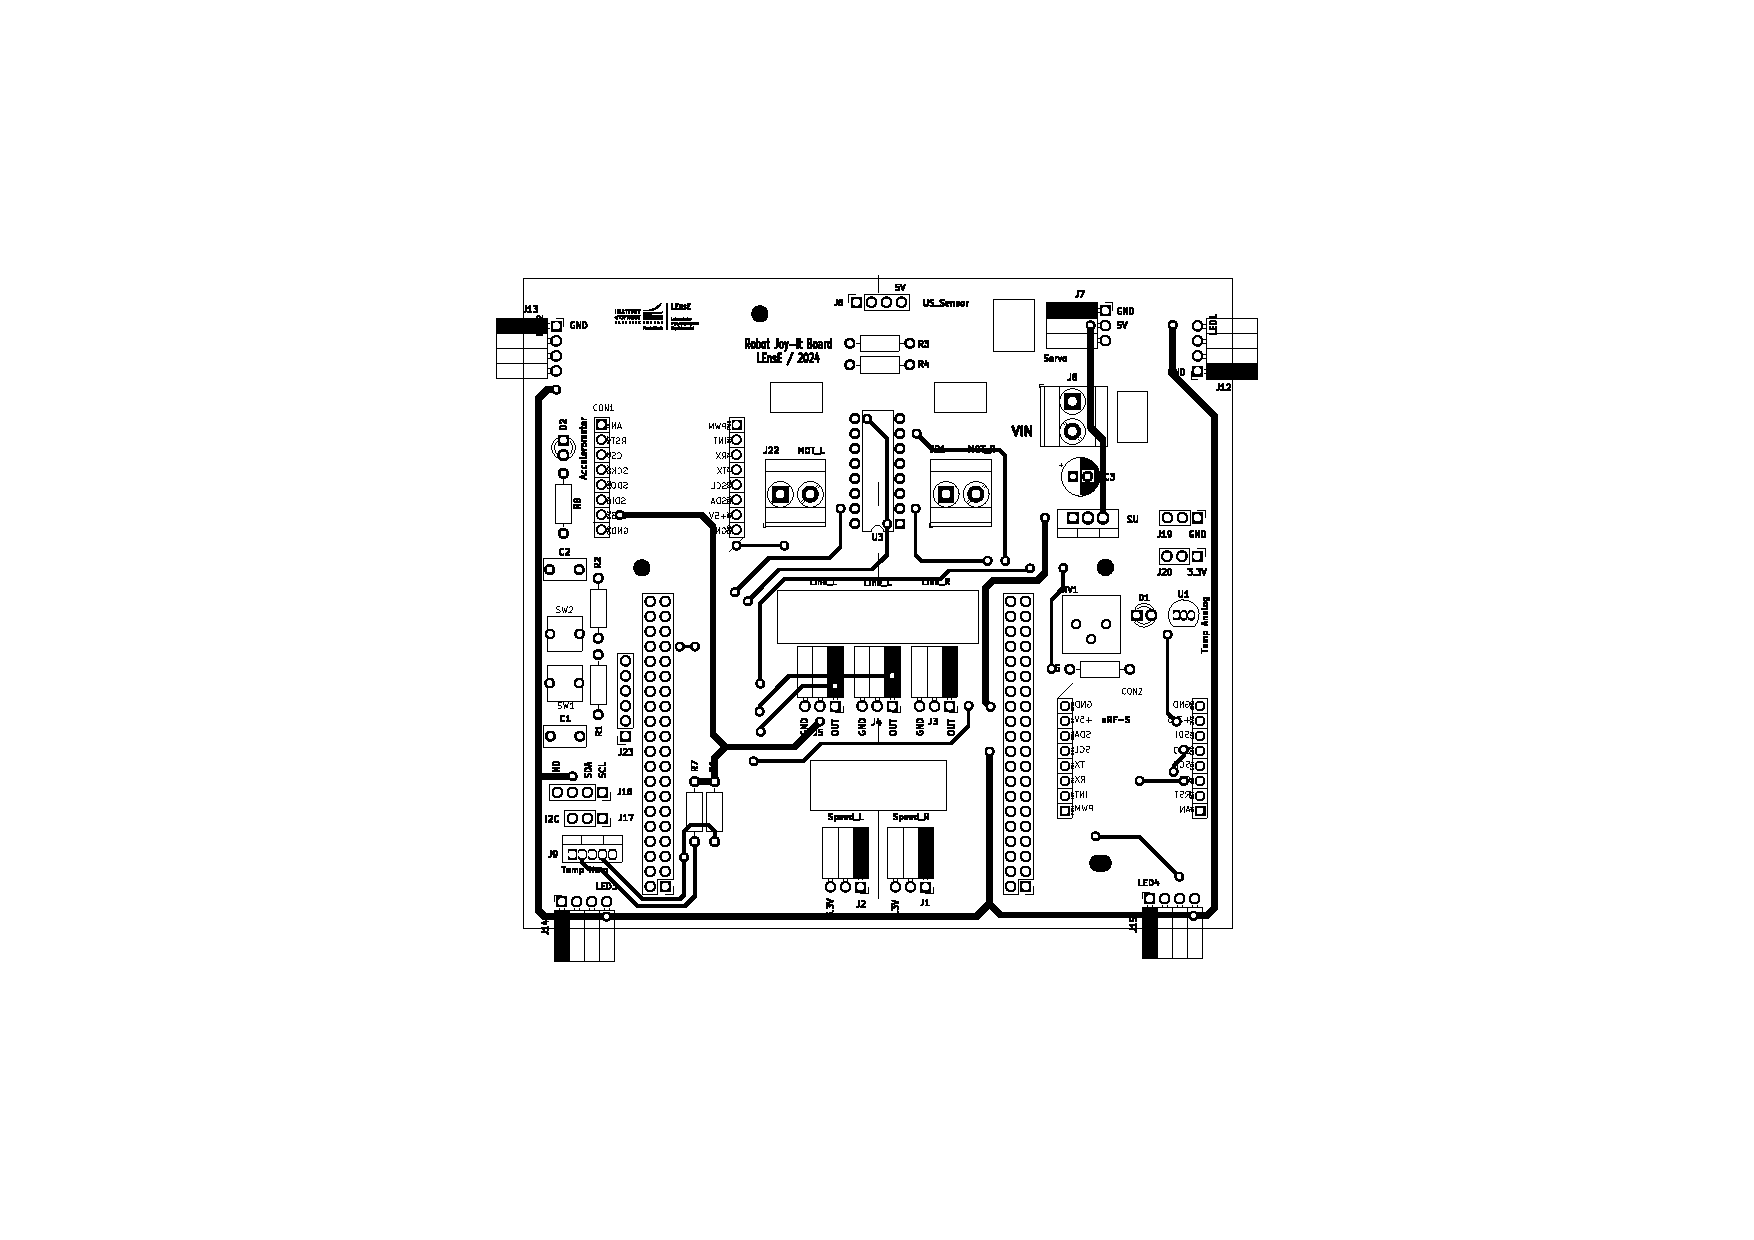
\includepdf[pages=1, landscape=true, pagecommand={\section{\texorpdfstring{\hspace{-1em}}{PCB Robot}}}\label{doc:robot_pcb}]{ressources/Motor_Board_L476RG_pcb.pdf}


\end{document}


